%!TEX TS-program = xelatex
\documentclass[notes,12pt, aspectratio=169]{beamer}

\usepackage{amsmath,amsfonts,amssymb,amsthm,mathtools}  % пакеты для математики
\usepackage{minted}

\usepackage[english, russian]{babel} % выбор языка для документа
\usepackage[utf8]{inputenc} % задание utf8 кодировки исходного tex файла
\usepackage[X2,T2A]{fontenc}        % кодировка

\usepackage{fontspec}         % пакет для подгрузки шрифтов
\setmainfont{Helvetica}  % задаёт основной шрифт документа

% why do we need \newfontfamily:
% http://tex.stackexchange.com/questions/91507/
\newfontfamily{\cyrillicfonttt}{Helvetica}
\newfontfamily{\cyrillicfont}{Helvetica}
\newfontfamily{\cyrillicfontsf}{Helvetica}

\usepackage{unicode-math}     % пакет для установки математического шрифта
% \setmathfont{Neo Euler} % шрифт для математики

\usepackage{polyglossia}      % Пакет, который позволяет подгружать русские буквы
\setdefaultlanguage{russian}  % Основной язык документа
\setotherlanguage{english}    % Второстепенный язык документа

% Шрифт для кода
\setmonofont[Scale=0.85]{Monaco}
\usepackage{verbments}

\usepackage{pgfpages}
% These slides also contain speaker notes. You can print just the slides,
% just the notes, or both, depending on the setting below. Comment out the want
% you want.
%\setbeameroption{hide notes} % Only slide
%\setbeameroption{show only notes} % Only notes
%\setbeameroption{show notes on second screen=right} % Both

\usepackage{array}

\usepackage{tikz}
\usepackage{verbatim}
\setbeamertemplate{note page}{\pagecolor{yellow!5}\insertnote}
\usetikzlibrary{positioning}
\usetikzlibrary{snakes}
\usetikzlibrary{calc}
\usetikzlibrary{arrows}
\usetikzlibrary{decorations.markings}
\usetikzlibrary{shapes.misc}
\usetikzlibrary{matrix,shapes,arrows,fit,tikzmark}

\usepackage{hyperref}
\usepackage{lipsum}
\usepackage{multimedia}
\usepackage{multirow}
\usepackage{dcolumn}
\usepackage{bbm}
\newcolumntype{d}[0]{D{.}{.}{5}}

\usepackage{changepage}
\usepackage{appendixnumberbeamer}
\newcommand{\beginbackup}{
   \newcounter{framenumbervorappendix}
   \setcounter{framenumbervorappendix}{\value{framenumber}}
   \setbeamertemplate{footline}
   {
     \leavevmode%
     \hline
     box{%
       \begin{beamercolorbox}[wd=\paperwidth,ht=2.25ex,dp=1ex,right]{footlinecolor}%
%         \insertframenumber  \hspace*{2ex} 
       \end{beamercolorbox}}%
     \vskip0pt%
   }
 }
\newcommand{\backupend}{
   \addtocounter{framenumbervorappendix}{-\value{framenumber}}
   \addtocounter{framenumber}{\value{framenumbervorappendix}} 
}

% для имитации питоновского синтаксиса 
\newcommand{\pgr}[1]{{\color{green} \textbf{#1}}}


%%%%%%%%%% Работа с картинками %%%%%%%%%
\usepackage{graphicx}                  % Для вставки рисунков
\usepackage{graphics}
\graphicspath{{images/}}    % можно указать папки с картинками
\usepackage{wrapfig}                   % Обтекание рисунков и таблиц текстом

\usepackage[space]{grffile}
\usepackage{booktabs}

% These are my colors -- there are many like them, but these ones are mine.
\definecolor{blue}{RGB}{0,114,178}
\definecolor{red}{RGB}{213,94,0}
\definecolor{yellow}{RGB}{240,228,66}
\definecolor{green}{RGB}{0,128, 0}

\hypersetup{
  colorlinks=false,
  linkbordercolor = {white},
  linkcolor = {blue}
}


%% I use a beige off white for my background
\definecolor{MyBackground}{RGB}{255,253,218}

%% Uncomment this if you want to change the background color to something else
%\setbeamercolor{background canvas}{bg=MyBackground}

%% Change the bg color to adjust your transition slide background color!
\newenvironment{transitionframe}{
  \setbeamercolor{background canvas}{bg=yellow}
  \begin{frame}}{
    \end{frame}
}

\setbeamercolor{frametitle}{fg=blue}
\setbeamercolor{title}{fg=black}
\setbeamertemplate{footline}[frame number]
\setbeamertemplate{navigation symbols}{} 
\setbeamertemplate{itemize items}{-}
\setbeamercolor{itemize item}{fg=blue}
\setbeamercolor{itemize subitem}{fg=blue}
\setbeamercolor{enumerate item}{fg=blue}
\setbeamercolor{enumerate subitem}{fg=blue}
\setbeamercolor{button}{bg=MyBackground,fg=blue,}


% If you like road maps, rather than having clutter at the top, have a roadmap show up at the end of each section 
% (and after your introduction)
% Uncomment this is if you want the roadmap!
% \AtBeginSection[]
% {
%    \begin{frame}
%        \frametitle{Roadmap of Talk}
%        \tableofcontents[currentsection]
%    \end{frame}
% }
\setbeamercolor{section in toc}{fg=blue}
\setbeamercolor{subsection in toc}{fg=red}
\setbeamersize{text margin left=1em,text margin right=1em} 

% списки, которые растягиваются на всю величину слайда 
\newenvironment{wideitemize}{\itemize\addtolength{\itemsep}{10pt}}{\enditemize}

\usepackage{ulem}

\title[]{\textcolor{blue}{Практический анализ данных и машинное обучение: искусственные нейронные сети}}
\author{Ульянкин Филипп}
\date{\today}


\begin{document}

%%% TIKZ STUFF
\tikzset{   
        every picture/.style={remember picture,baseline},
        every node/.style={anchor=base,align=center,outer sep=1.5pt},
        every path/.style={thick},
        }
\newcommand\marktopleft[1]{%
    \tikz[overlay,remember picture] 
        \node (marker-#1-a) at (-.3em,.3em) {};%
}
\newcommand\markbottomright[2]{%
    \tikz[overlay,remember picture] 
        \node (marker-#1-b) at (0em,0em) {};%
}
\tikzstyle{every picture}+=[remember picture] 
\tikzstyle{mybox} =[draw=black, very thick, rectangle, inner sep=10pt, inner ysep=20pt]
\tikzstyle{fancytitle} =[draw=black,fill=red, text=white]
%%%% END TIKZ STUFF

% Title Slide
\begin{frame}
\maketitle
\centering Обзор современных архитектур
\end{frame}


\begin{frame} {Agenda} 
\begin{wideitemize}
	\item   Частичное обучение
	\item   Как делать разметки 
	\item   Нейробайесовские методы (это никак не связано с частичным обучением, у нас два разных сюжета!)
\end{wideitemize}
\end{frame}


 \begin{transitionframe}
	\begin{center}
		\Huge Частичное обучение
	\end{center}
\end{transitionframe}


\begin{frame}{Задача частичного обучения}
\begin{wideitemize}
	\item У нас есть размеченная выборка $X^l$, для которой известны ответы $y^l$
	\item Кроме неё есть большой неразмеченный  кусок $X^k$
	\item Обычно неразмеченный кусок гораздо больше размеченного, так как у нас мало модераторов, хочется как-то использовать его при обучении
\end{wideitemize}
\end{frame}


\begin{frame}{Задача частичного обучения не сводится к классификации}
\begin{center}
	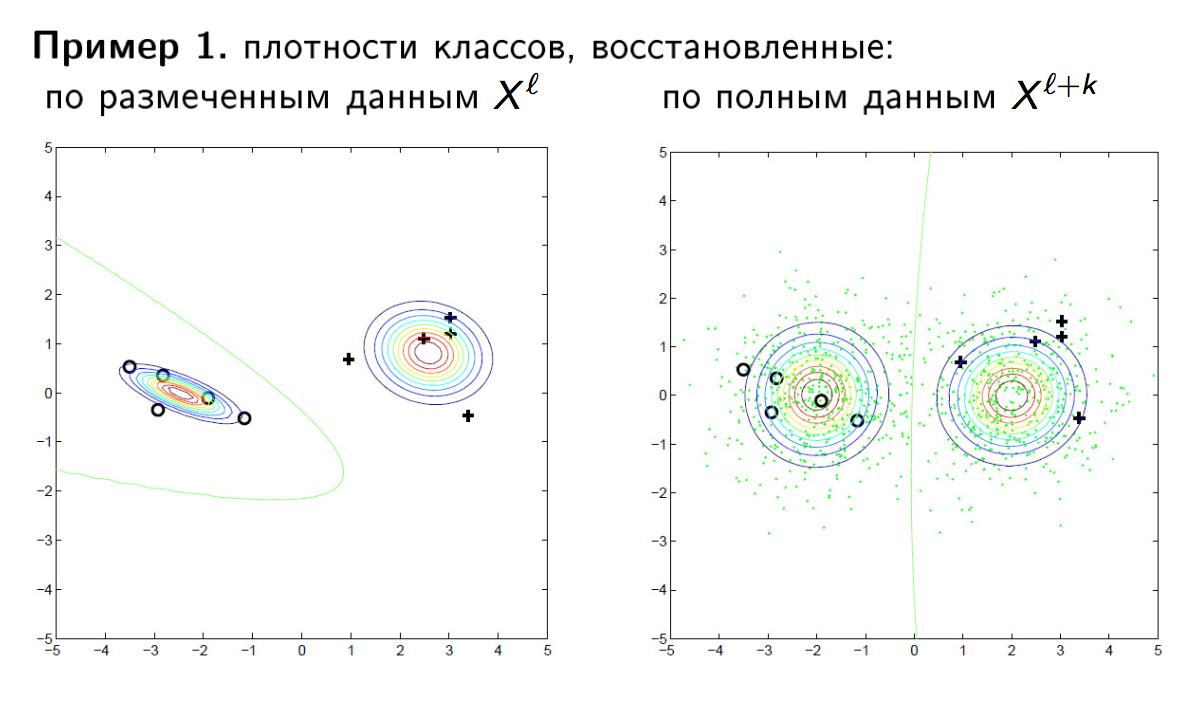
\includegraphics[width=.75\linewidth]{ex_1.png}
\end{center}
\end{frame}

\begin{frame}{Задача частичного обучения не сводится к классификации}
\begin{center}
	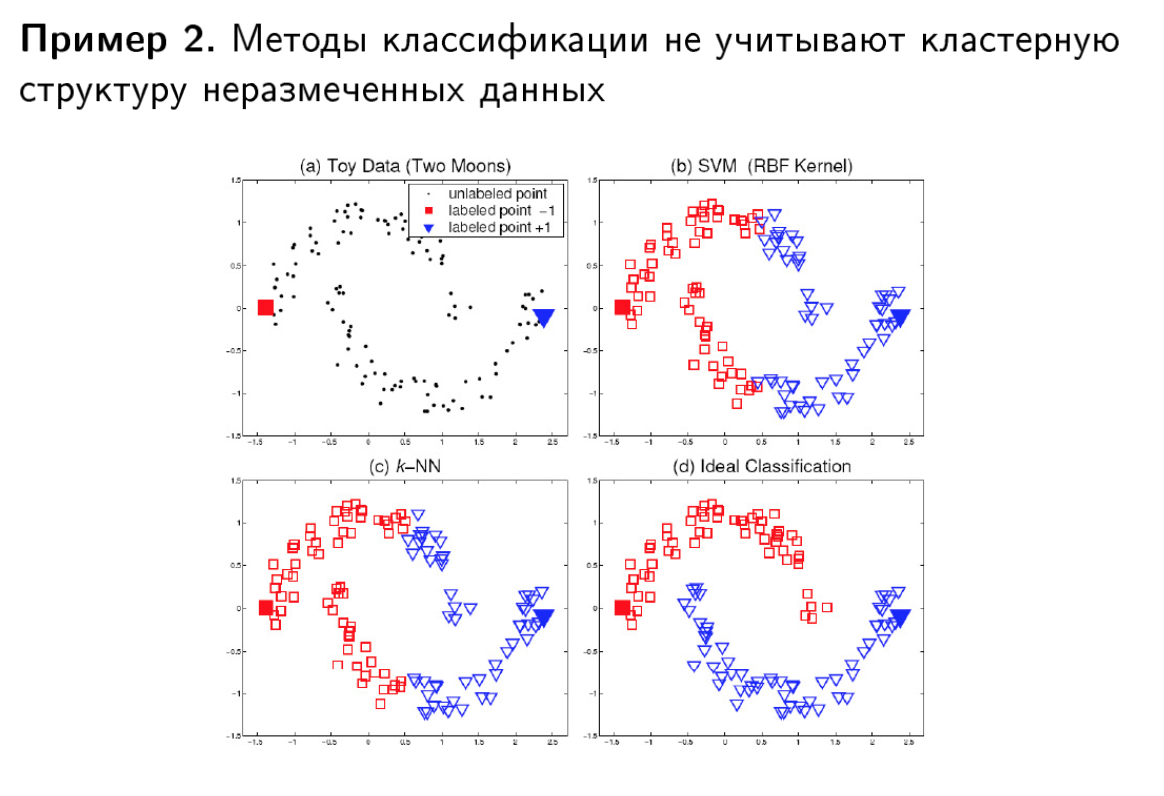
\includegraphics[width=.7\linewidth]{ex_2.png}
\end{center}
\end{frame}


\begin{frame}{Задача частичного обучения не сводится к кластеризации}
\begin{center}
	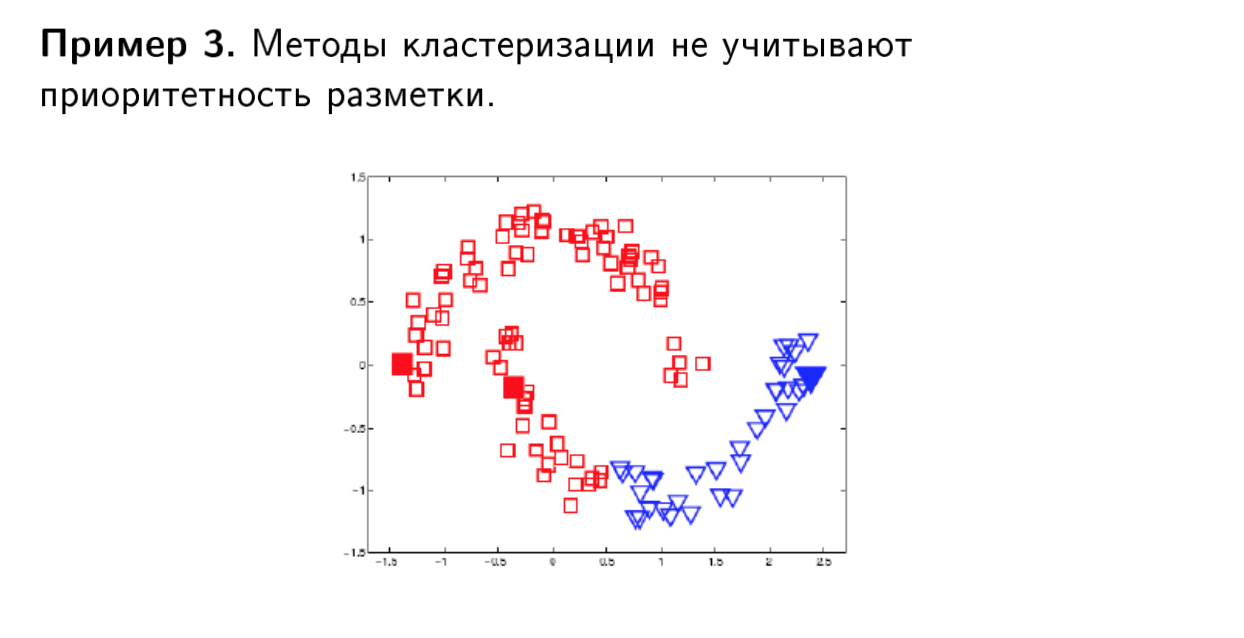
\includegraphics[width=.75\linewidth]{ex_3.png}
\end{center}
\end{frame}



 \begin{transitionframe}
	\begin{center}
		\Huge Простые обёртки над моделями
	\end{center}
\end{transitionframe}


\begin{frame}{Self-training (1965)}
\begin{wideitemize}
	\item Пусть $a(x)$ - наш алгоритм классификации, он выдаёт на выход степень уверенности $a_i = a(x_i)$ (например, вероятности)
	\item Простейший вариант дополнить разметку следующий: 
	
	\begin{enumerate}
		\item Учим $a(x)$ на $X^l$ и $y^l$
		\item Строим прогнозы для $X^k$
		\item Берём все объекты, где $a_i > M_0$ и добавляем их в обучающую выборку с меткой $1$, отсекая с другой стороны получаем объекты с меткой $0$
		\item Заново обучаем алгоритм $a(x)$, повторяем пока не надоест 
		\item $M_0$ - гиперпараметр 	
	\end{enumerate}
\end{wideitemize}
\end{frame}


\begin{frame}{Co-training (1998)}
\begin{wideitemize}
\item Пусть $a_1(x)$ и $a_2(x)$ два очень разных алгоритма, которые используют 

\begin{itemize} 
	\item  либо разные признаки;
	
	\item  либо разные парадигмы обучения
	
	\item либо разные источники данных  $X_1^{l_1}$, $X_2^{l_2}$
\end{itemize}

\item Схема обучения: 

\begin{enumerate}
	\item  Обучаем первый алгоритм на своей подвыборке

	\item Строим прогнозы $a_1(x)$ для $X^k$

	\item Все наблюдения, где $a_1(x) > M_0$ закидываем в выборку для второго алгоритма
		
	\item 	Обучаем второй алгоритм на его подвыборке 
	
	\item строим прогнозы $a_2(x)$ для $X^k$
	
	\item Все наблюдения, где $a_2(x) > M_0$ закидываем в выборку для первого алгоритма 
	
	\item Повторяем, пока не надоест
\end{enumerate}
\end{wideitemize}
\end{frame}


\begin{frame}{Co-learning (1993)}
\begin{wideitemize}
	\item Это self-training для композиции алгоритмов
	
	\item Решение брать или не брать наблюдение в обучающую выборку принимается на основе голосования композицией алгоритмов
\end{wideitemize}
\end{frame}

 \begin{transitionframe}
	\begin{center}
		\Huge От кластеризации к частичному обучению
	\end{center}
\end{transitionframe}

\begin{frame}{Кластеризация как задача дискретной оптимизации}
\begin{wideitemize}
	\item  Пусть $\rho(x, x')$ - функция расстояния между объектами, а $w_{ij} = exp(- \beta \rho(x_i,x_j))$ - веса на парах объектов (близости), где $\beta$ - параметр
	
	\item \alert{Задача кластеризации:} 
	
	$$
	\sum_{i,j} w_{ij} \cdot [a_i \ne a_j] \to \min_{a_i \in Y}
	$$
	
		\item \alert{Задача частичного обучения:} 
	
	$$
	\sum_{i,j} w_{ij} \cdot [a_i \ne a_j] {\color{red} + \lambda \cdot \sum_{i=1}^l [a_i \ne y_i] } \to \min_{a_i \in Y}
	$$
	
	\item То есть мы решаем задачу кластеризации и накладываем штраф на неверную кластеризацию объектов с известными классами
\end{wideitemize}
\end{frame}


\begin{frame}{Мораль}
Надо просто взять алгоритм кластеризации и модернизировать его так, чтобы был штраф в объектах с известными классами!
\end{frame}


\begin{frame}{Модернизация графовой кластеризации}

Пусть мы хотим раздробить выборку на $K$ кластеров, тогда алгоритм графовой кластеризации выглядел бы так: 

\begin{enumerate}
	\item Найти пару вершин $(x_i, x_j)$ с наименьшим расстоянием между ними и соединить ребром
	\item Пока  выборке остаются изолированные точки, находим изолированную точку и соединяем её с ближайшей 
	\item В итоге у нас получается остовное  дерево 
	\item Удалим из дерева $K-1$ самых длинных ребер
\end{enumerate}
\end{frame}

\begin{frame}{Модернизация графовой кластеризации}

Для перехода к задаче частичного обучения надо немного поменять последний шаг 

\begin{enumerate}
	\item Найти пару вершин $(x_i, x_j)$ с наименьшим расстоянием между ними и соединить ребром
	\item Пока  выборке остаются изолированные точки, находим изолированную точку и соединяем её с ближайшей 
	\item В итоге у нас получается остовное  дерево 
	\item \sout{Удалим из дерева $K-1$ самых длинных ребер}
	\item {\color{red} Пока есть путь между двумя вершинами разных классов, будем удалять на этом пути самое длинное ребро}
\end{enumerate}
\end{frame}

\begin{frame}{Модернизация иерархической кластеризации}

\begin{enumerate}
	\item Все классы 1 -элементные
	\item Ищем пары кластеров с минимальным расстоянием между ними и сливаем, пока все объекты не сольются в единый кластер 
	\item Считать расстояния между кластерами можно по-разному  
\end{enumerate}
\end{frame}

\begin{frame}{Модернизация иерархической кластеризации}

\begin{enumerate}
	\item Все классы 1 -элементные
	\item Ищем пары кластеров с минимальным расстоянием между ними и сливаем, пока все объекты не сольются в единый кластер, {\color{red} следим за тем, чтобы при слиянии не было объектов с разными метками классов} 
	\item Считать расстояния между кластерами можно по-разному  
\end{enumerate}
\end{frame}


 \begin{transitionframe}
	\begin{center}
		\Huge От классификации к частичному обучению
	\end{center}
\end{transitionframe}


\begin{frame}{От SVM к частичному обучению}
\begin{wideitemize}
\item 	В случае SWM мы пытаемся сделать разделяющую полосу как можно шире, для этого мы минимизируем функцию: 

$$
\sum_{i=1}^l (1 - M_i(w,w_0))_{+} + \frac{1}{2c} ||w||^2 \to \min_{w, w_0}
$$
	
\item Функция $L(M) = (1 - M)_{+}$ штрафует за уменьшение отступа

\item \alert{Идея!} Функция $L(M) = (1 - |M|)_{+}$ для объектов без метки будет штрафовать за попадание в зазор между классами	
\end{wideitemize}
\end{frame}


\begin{frame}{Transductive SVM}
\begin{wideitemize}
	\item  Обучение весов можно провести по частично размеченной выборке: 
	
	$$
	\sum_{i=1}^l (1 - M_i(w,w_0))_{+} + \frac{1}{2c} ||w||^2  { \color{red} + \gamma \cdot \sum_{i = 1}^k (1 - |M_i(w,w_0)|)_{+}	
}
	\to \min_{w, w_0}
	$$

	\item Гиперпараметр $\gamma$ отвечает за то, насколько много внимания мы уделяем не размеченной части 
	
	\item Если в выборке нет области разреженности, решение будет неустойчивым
\end{wideitemize}
\end{frame}


\begin{frame}{От логрегрессии к частичному обучению}
\begin{wideitemize}
	\item Обучение логрегрессии происходит в результате максимизации правдоподобия: 

$$
\sum_{i=1}^l \ln P(y_i \mid x_i, w) - \frac{1}{2C} \sum_{y \in Y} ||w_y||^2 \to \max_{w}
$$

	\item Функция выше для мультиклассовой задачи, если вы ещё не забыли, там у каждого класса свои веса, $P(y \mid x, w)$ - это softmax 
	
	\item Нам нужно учесть в этом функционале неразмеченные данные 
\end{wideitemize}
\end{frame}



\begin{frame}{От логрегрессии к частичному обучению}
\begin{wideitemize}
	\item Пусть $b_j(x)$ - бинарные признаки, $j = 1, \ldots, m$.

	\item Для неразмеченных объектов оценим $P(y \mid b_j(x = 1))$ двумя способами: 
	
	\begin{enumerate}
		\item  Эмпирическая оценка по размеченным данным $X^l$

$$
\hat p_j(y) = \frac{\sum_{i=1}^l b_j(x_i) [y_i = y]}{\sum_{i=1}^l b_j(x_i)}
$$

		
		\item  Оценка по неразмеченным данным $X^k$ и линейной модели: 
		
$$
\hat p_j(y) = \frac{\sum_{i=1}^k b_j(x_i) \cdot P(y \mid x_i, w)}{\sum_{i=1}^k b_j(x_i)}
$$		
		\item Хочется, чтобы эти две вероятности были похожи
	\end{enumerate}
	
\end{wideitemize}
\end{frame}


\begin{frame}{От логрегрессии к частичному обучению}
\begin{wideitemize}

\item Расстояние между распределениями измеряет $KL$-дивергенция, будем её минимизировать 

$$
KL(\hat p_j(y) || p_j(y, w)) = \sum_y \hat p_j(y) \cdot \ln \frac{\hat p_j(y)}{p_j(y,w)} \to \min_w 
$$

\item Итоговый функционал получается, если вычесть KL-дивергенцию, посчитанную по всем $m$ признакам из правдоподобия c коэффициентом $\gamma$

$$
\sum_{i=1}^l \ln P(y_i \mid x_i, w) - \frac{1}{2C} \sum_{y \in Y} ||w_y||^2 - \gamma \cdot \sum_{j=1}^m \sum_{y \in Y} \hat p_j(y) \cdot \ln \frac{\hat p_j(y)}{p_j(y,w)}  \to \max_{w}
$$

\end{wideitemize}
\end{frame}

\begin{frame}{От логрегрессии к частичному обучению}
\begin{wideitemize}
\item Оптимизация идёт методом стохастического градиентного спуска 

\item Метод слабо чувствителен к выбору $C$ и $\gamma$ 

\item Метод устойчив к погрешностям оценивания $\hat p_j(y)$

\item Не требует большого числа размеченных объектов, хорошо подходит для текстов, показывает неплохую точность 

\item Пример бинаризации $b_j(x)$ для текстов: [термин $j$ входит в текст $x$]

\end{wideitemize}
\end{frame}

\begin{frame}{Частичное обучение}
\begin{wideitemize}
	\item Задача занимает промежуточное положение между классификацией и кластеризацией, но не сводится к ним. 
	
	\item Простые методы-обёртки требуют многократного обучения
	
	\item Методы кластеризации легко адаптировать к частичному обучению, введением ограничений (constrained clustering), но это обычно вычислительно сложно 
	
	\item Методы классификации можно адаптировать чуть сложнее, но это приводит к более эффективному частичному обучению 
\end{wideitemize}
\end{frame}


 \begin{transitionframe}
	\begin{center}
		\Huge  Как делать разметки?
	\end{center}
\end{transitionframe}


\begin{frame}{Как создать свой датасет с Киркоровым и Фейсом}
\begin{center}
	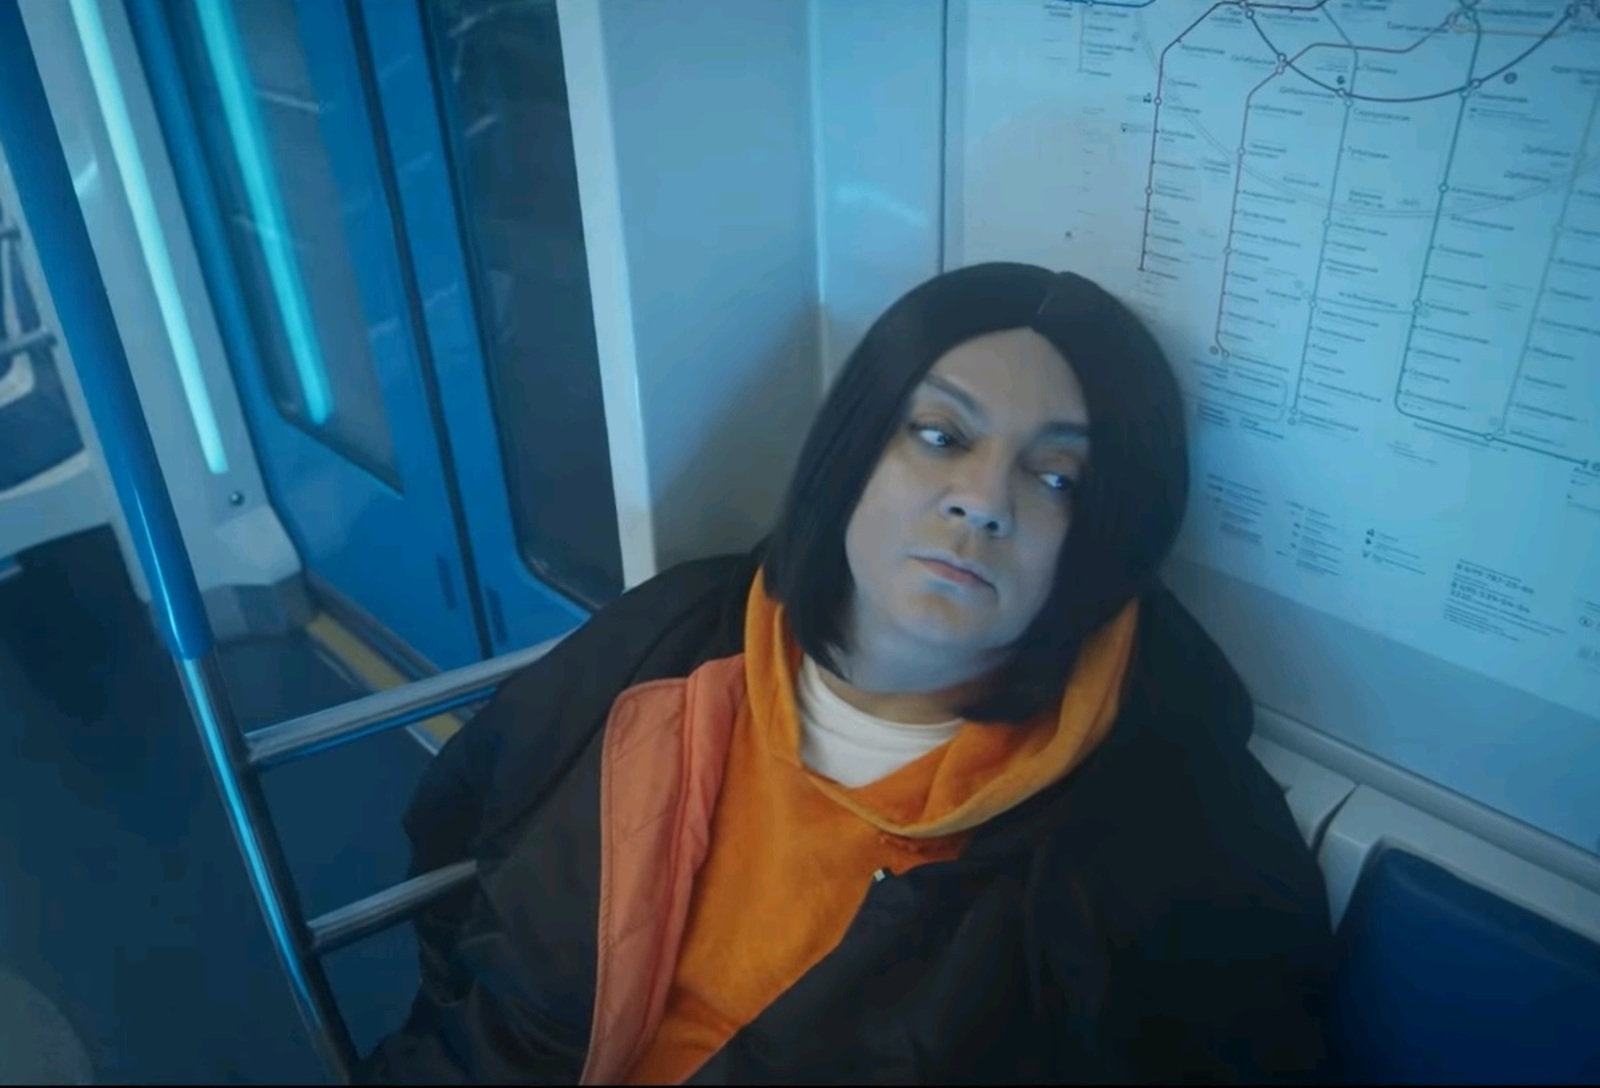
\includegraphics[width=.6\linewidth]{kirk.jpeg}
\end{center}

\vfill 

{\color{blue} \url{https://habr.com/ru/company/ods/blog/358574/} }
\end{frame}



\begin{frame}{Что я понял, работая в Data science}
\begin{wideitemize}
	\item Разметок мало, они плохие \pause 
	
	\item Люди - сволочи \pause 
	
	\item Толокеры не читают инструкцию, приходится делать на проектах обучение и экзамены \pause 
	
	\item  Люди - жадные сволочи \pause 
	
	\item Толокеры хотят побольше денег просто так, приходится следить за качеством разметки, делать ханипоты (примеры, ответы на которые мы знаем), выгонять толокеров, если они делают разметку недобросовестно  \pause 
\end{wideitemize}
\end{frame}
	
\begin{frame}{Что я понял, работая в Data science}
\begin{wideitemize}
	\item Люди - жадные сволочи, которые умеют учиться \pause 
	
	\item Ханипоты приходится обновлять, для этого нужны отдельные процессы \pause 
	
	\item  Люди - тупые жадные сволочи, которые умеют учиться \pause 
	
	\item Чем больше вопросов в разметке, тем хуже итоговые результаты

\end{wideitemize}
\end{frame}



 \begin{transitionframe}
	\begin{center}
		\Huge  Нейробайесовские методы
	\end{center}
\end{transitionframe}

\begin{frame}
\begin{center}
	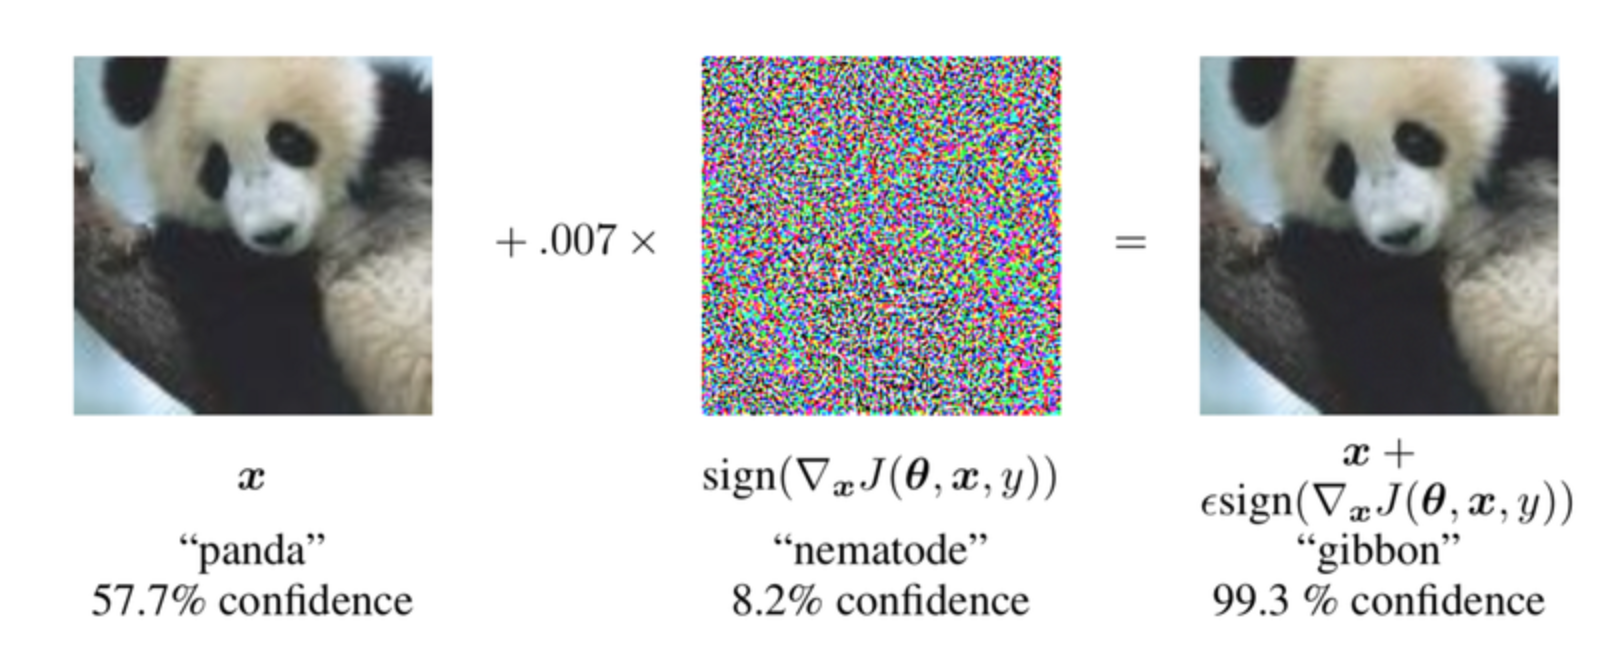
\includegraphics[width=.9\linewidth]{panda.png}
\end{center}

\vfill 

{\color{blue} \url{https://www.youtube.com/watch?v=kFe5zSkro0E} }
\end{frame}

\begin{frame}{Байесовский w2v}
\begin{wideitemize}
	\item ватерло - лондон - станция - поезд 
	\item ватерло - наполеон - аустерлиц - битва 
	\item ватерло - абба - мама-миа
\end{wideitemize}
\end{frame}

\begin{frame}{Байесовский w2v}
\begin{wideitemize}
	\item S. Bartunov, D. Kondrashkin, A. Osokin, D. Vetrov. Breaking Sticks and
Ambiguities with Adaptive Skip-gram. In AISTATS 2016 {\color{blue} \url{http://arxiv.org/abs/1502.07257}}

	\item Код и документация: {\color{blue} \url{https://github.com/sbos/AdaGram.jl}}
	
	\item Предобученная модель: {\color{blue} \url{https://yadi.sk/d/W4FtSjA5o3jUL} }
\end{wideitemize}
\end{frame}


\begin{frame}
\begin{center}
	
\includegraphics[width=.6\linewidth]{end.jpg}
\end{center}
\end{frame}


\end{document}
